\documentclass[journal]{IEEEtran}
% *** GRAPHICS RELATED PACKAGES ***
\ifCLASSINFOpdf
  \usepackage[pdftex]{graphicx}
\else
  \usepackage[dvips]{graphicx}
\fi
\usepackage{float}
% *** MATH PACKAGES ***
\usepackage[cmex10]{amsmath}

\begin{document}
%
% paper title
\title{Decodificaci\'{o}n MPEG2}
\author{Alberto~Suarez,~\IEEEmembership{Ingeniero,~Hewlett~Packard,}
        Yu~Shan~Hsieh,~\IEEEmembership{Ingeniero,~Hewlett~Packard}% <-this % stops a space
\thanks{}% <-this % stops a space
}
% make the title area
\maketitle

% in the abstract or keywords.
\begin{abstract}
Art\'{i}culo cient\'{i}fico sobre benchmarking en la decodificaci\'{o}n de mpeg2.
\end{abstract}

% Note that keywords are not normally used for peerreview papers.
\begin{IEEEkeywords}
Decodificaci\'{o}n, mpeg2, Benchmark
\end{IEEEkeywords}

\section{Introducci\'{o}n}
\IEEEPARstart{E}{l} prop\'{o}sito de este paper es analizar varios aspectos de rendimiento que tiene un programa de decodificaci\'{o}n de mpeg2 tales como consumo de potencia, desempe\~{n}o de la CPU, tiempo de ejecuci\'{o}n, etc. 
Para poder hablar sobre esos aspectos, es importante primero entender qu\'{e} es la decodificaci\'{o}n de mpeg2 y c\'{o}mo se realiza. Para esto se analizar\'{a} los c\'{o}digos fuentes que  Posteriormente se detallar\'{a} las pruebas que se van a realizar y el testbench sobre la cual se realizar\'{a} las pruebas. Luego que har\'{a} el an\'{a}lisis de resultados y finalmente las conclusiones que se pueden derivar de estos experimentos.


\hfill Setiembre 27, 2013

\section{Metodolog\'{i}a de optimizaci\'{o}n}

\subsection{Descripci\'{o}n del benchmark}

\subsection{Herramientas}

\subsubsection{Simplescalar}
Simplescalar\cite{SIMPLESCALAR} es un simulador de arquitectura de computadoras Open Source escrito en C. Este simulador contiene una serie de herramientas que modela un sistema computador virtual con CPU, cache y jerarqu\'{i}as de memoria.
Utilizando Simplescalar, el usuario puede modelar lo que ocurre cuando un programa corre sobre una variedad de arquitecturas desde procesadores sencillos hasta procesadores con scheduling din\'{a}mico, cache no-bloqueante
y con predicci\'{o}n de saltos. Simplescalar soporta set de instrucciones tipo PISA y se compone de tres herramientas principales: \newline

\begin{itemize}
\item \textbf{simplesim} Simulador Simplescalar.
\item \textbf{simpletools} Compilador GNU GCC de PISA para Simplescalar.
\item \textbf{simpleutils} Herramientas para el compilador que incluyen el ensamblador de PISA, linker, etc. \newline
\end{itemize}

\subsubsection{Wattch}
Wattch\cite{WATTCH} es un simulador que estima la potencia consumida de un CPU. Tiene modelos de potencia integrados en Simplescalar y utiliza una version modificada de sim-outorder de Simplescalar para recolectar resultados. \newline

\subsubsection{GCC}
GNU Compiler Collection o GNU C Compiler es un compilador de C para sistemas operativos GNU. \newline

\subsubsection{Mpeg2 decoder}
El decodificador viene en un suite que trabaja tanto la parte de codificaci\'{o}n (encode) como la de decodificaci\'{o}n. En nuestro caso, solo vamos a trabajar la parte de decode.
Dentro del directorio de src/mpeg2dec se encuentra el codigo en C del decoder junto con el Makefile. El archivo principal es mpeg2dec.c y est\'{a} compuesto por las siguientes funciones principales:

\footnotesize \begin{verbatim}
static void Initialize_Decoder _ANSI_ARGS_((void));
static int Decode_Bitstream _ANSI_ARGS_((void));
\end{verbatim}
\normalsize

La funci\'{o}n de \textit{Decode\_Bitstream} llama a la funci\'{o}n video\_sequence() que se encarga de ir por cada imagen y decodificarlo. \newline

\subsection{Configuraci\'{o}n}
En esta secci\'{o}n se va a hace un an\'{a}lisis preliminar de la configuraci\'{o}n de la arquitectura (sistema de referencia a utilizar).

El c\'odigo de decodificaci\'on MPEG2 vemos que contiene en su mayor\'ia contiene variables de tipo integer, punteros y referencias a memoria para procesar los buffers de datos a decodificar. Existen apenas tres variables de tipo double, y se ejecutan unas cuantas operaciones con las mismas.  El codigo se basa en llamadas a funciones y luego a otras cuantas mas logrando cerca de unos 5 niveles de anidaci\'on de las llamadas, lo cual representan saltos multiples que pueden afectar el IPC.
Dedido a la muy poca utilizaci\'on de doubles se espera una poca utilizaci\'on de ALUs de punto flotante. \newline

\subsection{Funci\'{o}n Costo}
Definici\'{o}n de la funci\'{o}n costo.
Debido al uso tan extenso que se hace de la codificaci\'{o}n/decodificaci\'{o}n MPEG2, se opta por\
definir nuestra funci\'{o}n de costo en base al rendimiento del chip asi como la energ\'{i}a \
consumida por el mismo, ya que nos parece son los par\'{a}metros que se deber\'{i}an de maximisar para\
esta aplicaci\'{o}n.  El rendimiento es necesario para permitir una decodificaci\'{o}n r\'{a}pida y \
eficiente, la energ\'{i}a es importante por motivos del costo de consumo de la misma para \
realizar las decodificaciones.

\footnotesize \begin{verbatim}
Funcion de costo:     F(x) = P(x) * D(x)
P(x) = Potencia de x (Potencia total consumida por el chip)
D(x) = Rendimiento IPC del codigo.
\end{verbatim}
\normalsize

\subsection{EspacioDiseno}
Resultados preliminares y Espacio de Dise\~no.
De la primer corrida obtenemos los siguientes datos: \newline
\footnotesize \begin{verbatim}
Total Power Consumption: 56.2826
sim_IPC         1.8649 # instructions per cycle
sim_CPI         0.5362 # cycles per instruction
il1.misses      277707 # total number of misses
dl1.misses      96318 # total number of misses
ul2.misses      20691 # total number of misses
itlb.misses     32 # total number of misses
dtlb.misses     114 # total number of misses
il1.hits        178888369 # total number of hits
dl1.hits        32954311 # total number of hits
ul2.hits        384866 # total number of hits
itlb.hit        179166044 # total number of hits
dtlb.hits       33333723 # total number of hits
il1.miss_rate   0.0015 # miss rate (i.e., misses/ref)
dl1.miss_rate   0.0029 # miss rate (i.e., misses/ref)
ul2.miss_rate   0.0510 # miss rate (i.e., misses/ref)
itlb.miss_rate  0.0000 # miss rate (i.e., misses/ref)
dtlb.miss_rate  0.0000 # miss rate (i.e., misses/ref)
\end{verbatim}
\normalsize

Se aprecia que la cantidad de cache misses es muy peque\~na en comparaci\'on con los hits, todos lo miss rates son menores o iguales al 5 por ciento, dada esta caracter\'istica no nos vamos a enfocar en tratart de mejorar el hit rate de las caches, sino en intentar otras configuraciones para intertar bajar la potencia total y el CPI.
Dada la cantidad de saltos se opta por variar las politicas del branch predictor, la configuracion por default ya cuenta con suficientes ALUs para integers por lo que no vamos a intentar variar este componente.  Como se trabaja mucho con datos de memoria y punteros tambien se opta por variar los componenetes para actualizar los registros as\'i como el tama\~no del queue para los Loads y Stores.

Nuestro espacio de dise\~no va a ser entonces: branch preditor, el register update unit (RUU) size, load/store queue (LSQ) size, y la politica de reemplazo de bloques en las memorias cache(FIFO, LFU).

\subsection{Simulaciones a realizar}
C\'{a}lculo de la cantidad total de simulaciones a realizar.
Las simulaciones preliminares nos dan un estimado de 279 segundos para correr cada simulaci\'{o}n, \
lo cual corresponde aproximadamente a 4 minutos.  En un lapso de 45 minutos teoricamente se pueden correr alrededor de 11 simulaciones. Dado que son pocas las iteraciones que se pueden correr en un lapso de 45 minutos,
nos tenemos que limitar a correr 12 simulaciones, lo que implica que solo se van a probar 12 combinaciones posibles.
A continuaci\'{o}n se muestra las pruebas y su configuracion: \newline

\begin{enumerate}
\item \textbf{Test 1}.  bpredm=comb, lsq=8, ruu=16, cache=lfu
\item \textbf{Test 2}.  bpredm=comb, lsq=8, ruu=32, cache=lfu
\item \textbf{Test 3}.  bpredm=comb, lsq=8, ruu=32, cache=fifo
\item \textbf{Test 4}.  bpredm=comb, lsq=16, ruu=16, cache=lfu
\item \textbf{Test 5}.  bpredm=comb, lsq=16, ruu=32, cache=lfu
\item \textbf{Test 6}.  bpredm=comb, lsq=16, ruu=32, cache=fifo
\item \textbf{Test 7}.  bpredm=2lev, lsq=8, ruu=16, cache=lfu
\item \textbf{Test 8}.  bpredm=2lev, lsq=8, ruu=32, cache=lfu
\item \textbf{Test 9}.  bpredm=2lev, lsq=8, ruu=32, cache=fifo
\item \textbf{Test 10}. bpredm=2lev, lsq=16, ruu=16, cache=lfu
\item \textbf{Test 11}. bpredm=2lev, lsq=16, ruu=32, cache=lfu
\item \textbf{Test 12}. bpredm=2lev, lsq=16, ruu=32, cache=fifo \newline
\end{enumerate}

Las simulaciones se lanzan con el script \textit{./run\_benchmark.sh} que llama a Wattch junto con el binario cross-compilado de Simplescalar.

\subsection{Resultados}

\begin{figure}[!ht]
        \begin{center}
        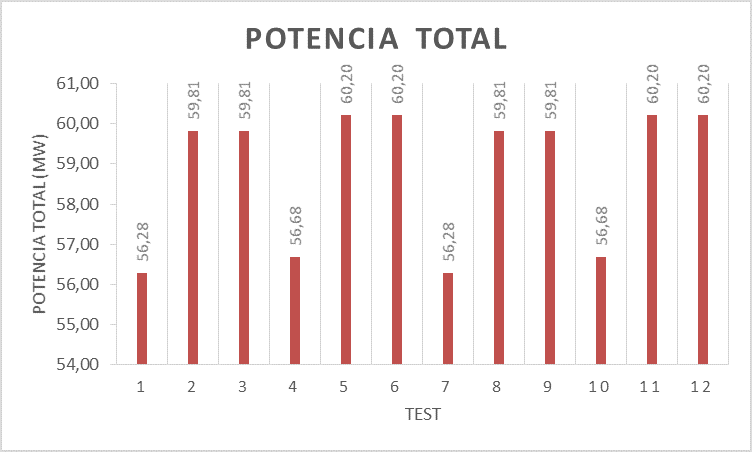
\includegraphics[width=3in]{fig1.png}
        \caption{Resultados de Potencia total}
        \end{center}
\end{figure}

\begin{figure}[!ht]
        \begin{center}
        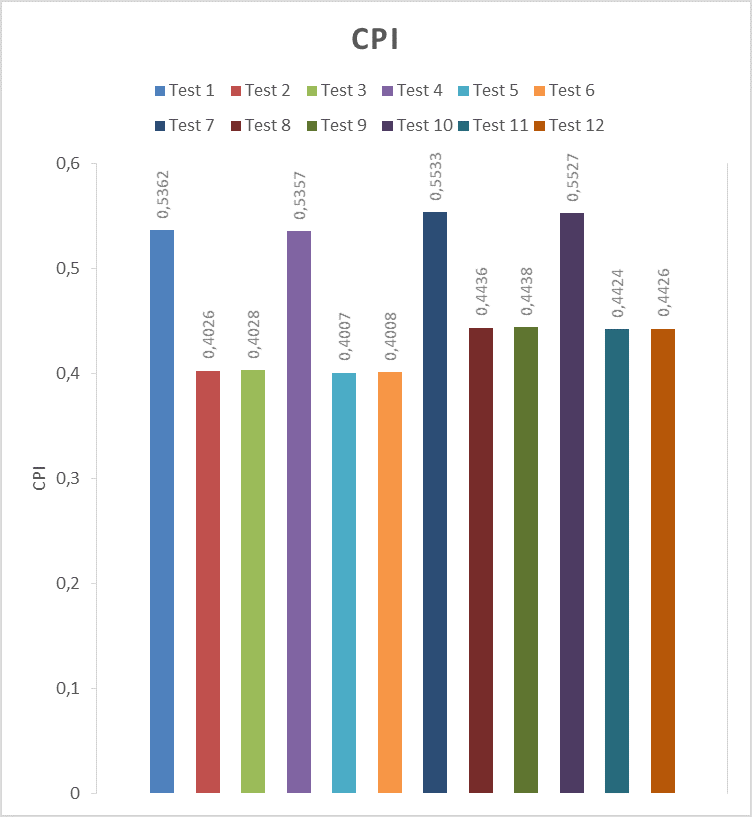
\includegraphics[width=3in]{fig2.png}
        \caption{Resultados de IPC}
        \end{center}
\end{figure}

\begin{figure}[!ht]
        \begin{center}
        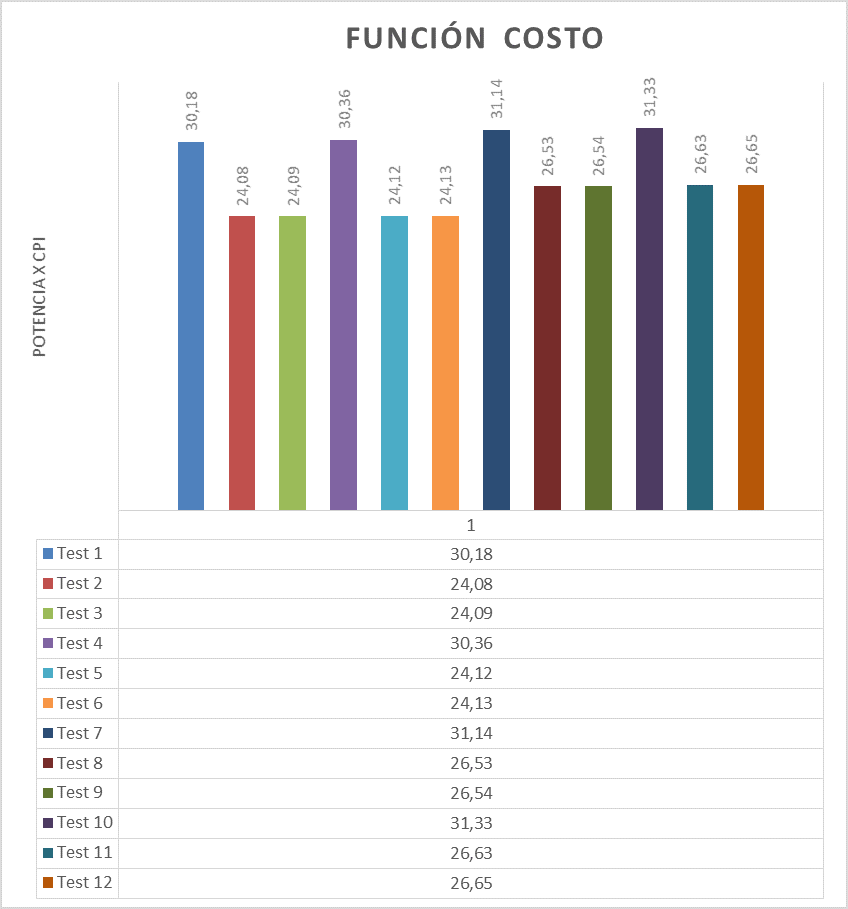
\includegraphics[width=3in]{fig3.png}
        \caption{Gr\'{a}fica de Funci\'{o}n Costo}
        \end{center}
\end{figure}

\subsection{An\'{a}lisis de Resultados}
A partir de los resultados se observa que al reducir el tama\~{n}o de la RUU se obtiene mejor potencia total (m\'{a}s baja). Esto es de imaginar ya que el algoritmo de decodificaci\'{o}n de mpeg2 hace bastante uso de de buffers y de operaciones en registros. Al mismo tiempo, al reducir la RUU de 32 a 16, aumenta la cantidad de ciclos necesarios para ejecutar una instrucci\'{o}n (CPI). Noten que este aumento en la CPI
tiene mayor peso sobre la funci\'{o}n costo que la potencia reducida. En otras palabras, la mejora que se obtuvo en potencia no fue lo suficiente para compensar el incremento en la CPI. Al incrementar la CPI se incrementa tambi\'{e}n
el tiempo de ejecuci\'{o}n del programa lo cual no es deseable.

El segundo factor que mas influenci\'{o} fue el modo del Branch Predictor, y las variables utilizadas son \textit{2Lev} y \textit{comb} con el \'{u}ltimo siendo el m\'{e}todo por default del compilador. Note con el m\'{e}todo \textit{comb} se produce
mejores tasas de CPI de forma consistente en comparaci\'{o}n con \textit{2Lev}.

Los cambios en la estrategia de reemplazo de los bloques de la cache y el tamaño del queue de LoadStore no aportan variaciones significativas de la funci\'{o}n costo aunque se observa una ligera mejora en la CPI al utilizar LFU en comparaci\'{o}n con utilizar FIFO. Esto se debe a que el c\'{o}digo hace un uso intensivo de la memoria y las acciones realizadas con estos datos permiten calendarizar otras operaciones entre lecturas de memoria.


Configuraci\'on optima:
bpred:comb
ruu:size
lsq:size
cache:dl1       dl1:128:32:4:l
cache:dl2       ul2:1024:64:4:l
cache:il1       il1:512:32:1:l

\section{Conclusiones}
Conclusiones.

% use section* for acknowledgement
\section*{Acknowledgment}

\begin{thebibliography}{1}
\bibitem{MPEG2-ENCODER/DECODER}
MPEG Software Simulation Group, MPEG-2 Encoder/Decoder, Version 1.2, July 19, 1996

\bibitem{SIMPLESCALAR}
Simplescalar LLC, http://www.simplescalar.com/, 2395 Timbercrest Court Ann Arbor, MI 48105

\bibitem{WATTCH}
Wattch, http://www.eecs.harvard.edu/~dbrooks/wattch-form.html, Version 1.02d.

\end{thebibliography}

\begin{IEEEbiographynophoto}{Alberto Suarez}
Ingeniero Electr\'{o}nico, Hewlett Packard
\end{IEEEbiographynophoto}

% if you will not have a photo at all:
\begin{IEEEbiographynophoto}{Yu Shan Hsieh}
Bachillerato en Ingenier\'{i}a El\'{e}ctrica, UCR
Ingeniero Electr\'{o}nico, Hewlett Packard
\end{IEEEbiographynophoto}

\end{document}


